\documentclass[11pt]{article}

\usepackage{amssymb,amsmath}
\usepackage{times,psfrag,epsf,epsfig,graphics,graphicx,caption}
\usepackage{enumitem,fontawesome}
\usepackage{algorithm}
\usepackage{algorithmic}

\begin{document}
\date{}

\title{PHSX 343: Assignment 12}

\author{William Jardee}

\maketitle


\section*{Problem 1}
    \begin{enumerate}[label=\alph*)]
    \item
        We can just use the $hf_{threshold} = \Phi$ and $f = \frac{c}{\lambda}$ to solve for all out values:
        \begin{center}
            $f_{threshold} = \frac{\Phi}{h} = \boxed{4.72 \times 10^{14} hz}$ and $\lambda _t = \frac{c}{f_{t}} = \boxed{635 nm}$
        \end{center}
    \item
        $eV_0 = hf - \Phi = \frac{hc}{\lambda} - \Phi$ where $\Phi = 1.95eV$, $hc = 1240eV\cdot nm$, and $\lambda = 300nm$.
        \[\boxed{eV = 2.18 eV}\]
    
    \end{enumerate}

\section*{Problem 2}

\begin{enumerate}[label=\alph*)]
    \item I plotted this with python, using the matplotlib.pyplot and numpy modules. the numpy modules allowed me to calculate the line of best fit exactly with what I gave it. Getting a rough estimate isn't hard by hand however; what you'd do is just just find the slope between the points and use point-intercept to find the intercept.\\
    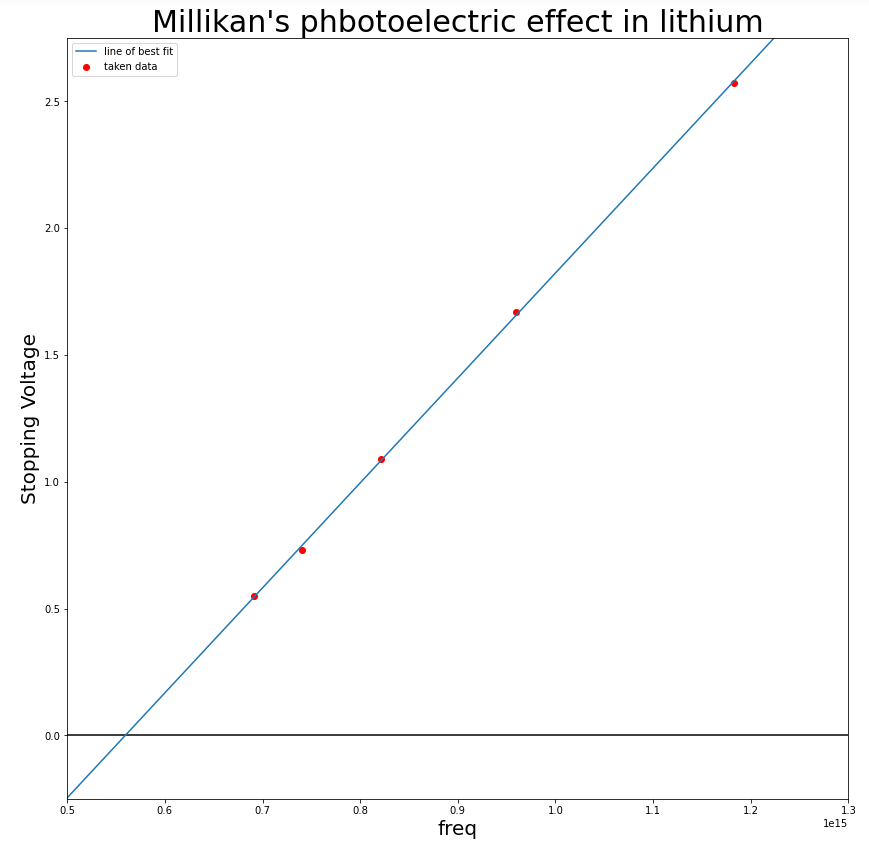
\includegraphics[width = \linewidth]{Homework12/question 2.PNG}\\
    Where the line is given by $V = 4.137 \times 10^{-15} f - 2.315$. This equation is equivalent to saying $V = hf -\Phi$. So:
    \begin{center}
        $\boxed{h = 4.14 \times 10^{-15}eV\cdot s}$ and $\boxed{\Phi = 2.32eV}$
    \end{center}
    The threshold frequency is given by the x-intercept. 
    \[0 = 4.137f-2.315 \rightarrow f = \frac{2.135}{4.137 \times 10^{-15}} =\boxed{ 5.59 \times 10^{14} hz}\]
    \item 
        We are looking for when $hf \geq 4.14$eV. If we multiply the array of frequencies given by h, we get
        \[[4.89, 3.97, 3.40, 3.06, 2.86]\]
        Only the first value is greater than 4.14, so only the first wavelength has enough energy to cause emission of photo electrons. The question asks for the converse though, so all but the first wavelength would not cause emission. 
\end{enumerate}

\section*{Problem 3}
    Using the outline of compton scattering from the lecture notes:
    \[\lambda _2 = \lambda _1 + \frac{hc}{mc^2}(1-cos(\theta)\]
    Using the values that $\theta = \frac{115\pi}{180} = 2.007$, $\lambda _1 = \frac{E}{hc} = 0.0024nm$, $hc = 1240eV \cdot nm$, $m = 0.511\frac{MeV}{c^2}$: $\lambda _2 = 0.0059 nm$. Recalculating this as the energy of the photon: $E_p = \frac{hc}{\lambda} = \boxed{0.211 MeV}$. Now, using conservation of energy: 
    \[E_e = E_{p_i} + mc^2 - E_{p_f} = \frac{hc}{\lambda _1} + mc^2 - \frac{hc}{\lambda _2} = \boxed{0.811 eV}\]
    Now to find the direction, we can use the $-\frac{h}{\lambda _2} sin(\theta) = p_e sin(\phi)$ equation.
    \[p_e = \sqrt{E^2 - (mc^2)^2} = 0.630 \frac{MeV}{c}\]
    \[\phi = sin^{-1}\Big(-\frac{hc}{\lambda _2 p_e}sin(\theta)\Big) = \boxed{-0.308} = -17.7^o\]
    
\section*{Problem 4}    
    First, to find what case gives us the maximum kinetic energy, let's set up the conservation of energy
    \[E_\gamma + mc^2 = E_{\gamma _f}+ E_{e_f} = E_{\gamma _f} + K + mc^2 \rightarrow E_\gamma = E_{\gamma _f} + K\]
    So what is $E_{\gamma _f}$? $E_{\gamma _f} = \frac{hc}{\lambda _2} = \frac{hc}{\lambda _1 + \frac{hc}{mc^2}(1-cos(\theta))}$. This value is minimized when $cos(\theta) = -1$ so the denominator in maximized. Obviously this is when $\theta = \pi$. So then:
    \begin{center}
    $K_{max} = E_\gamma -\frac{hc}{\lambda _1 +\frac{2hc}{mc^2}} = E_\gamma - \frac{E_\gamma}{1 + \frac{2E_\gamma}{mc^2}} = E_\gamma - \frac{E_\gamma mc^2 }{mc^2 + 2E_\gamma}$\\
    $K_{max} = \frac{E_\gamma mc^2 + 2E_\gamma ^2 -E_\gamma mc^2}{2E_\gamma + mc^2} = \frac{2E^2_\gamma}{2E_\gamma + mc^2}$\\
    \end{center}
    \begin{flushright}
\includegraphics[width = 70pt]{Homework12/thumpsup.jpg}
    \end{flushright}
    
    \newpage
    \[Q_{rad}^- + \begin{}\]
    
\end{document}
